\section{Comparison Matrix}

The following is a summary comparison of the vendors.

\begin{figure}
    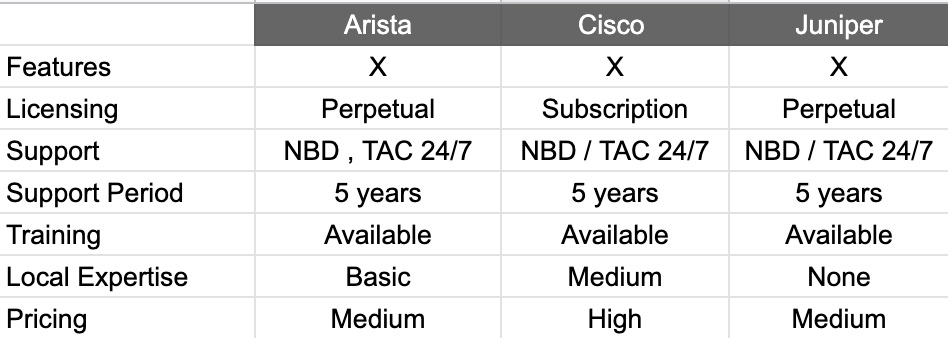
\includegraphics[width=11cm]{images/matrix.jpg}
    \centering
\end{figure}

All vendors met the technical requirements exposed in the network design. 

Cisco is the only vendor not offering a perpetual license; hence Cisco licenses must be renewed. 

Training is available for all vendors, but Juniper bundles an "All-Access Pass" for a year for a single person.

IT staff has plenty of experience with Cisco devices. Despite only a couple of Arista devices installed in Rubin's network, the expertise of Cisco can be extended to Arista, given that the interfaces are pretty similar. Regarding Juniper, Rubin Network engineers have no experience with it. 

Pricing details can be reviewed for each vendor; however, Cisco is the most expensive of them. 

All vendors offered five years of support which leaves Rubin well into operations. 

